\section{Messen von Induktivit\"aten}
Die Messung von Induktivit\"atswerten wird nach allen anderen Messungen als separater Teil mit allen
gefundenen Widerst\"anden mit weniger als \(2100~\Omega\) durchgef\"uhrt.
Das Messverfahren beruht auf dem Prinzip, dass beim Schliessen des Stromkreises der Strom nach
der Formel \(Il~=~Imax~\cdot~(1~-~\exp{\frac{-t}{\tau}})\) ansteigt.
Die Zeitkonstante \(\tau = \frac{L}{R}\) ist proportional zu der Induktivit\"at~\(L\), aber umgekehrt
proportional zum Widerstand~\(R\). 
Der Strom kann hier nur indirekt \"uber den Spannungsabfall an einem Widerstand
gemessen werden.
Leider wird durch den relativ hohen Widerstand \(680~\Omega\) die Zeitkonstante zus\"atzlich verringert, was
wiederum die Messung von kleinen Induktivit\"aten mit dem Takt von 8 MHz zus\"atzlich erschwert.
Um die Zeitkonstante zu bestimmen, wird die Spannung am \(680~\Omega\)-Widerstand als Stromsensor
mit dem analogen Komparator \"uberwacht. Wenn der Spannungsabfall am \(680~\Omega\)-Widerstand gr\"osser als
die Vergleichs-Spannung der internen Spannungsreferenz wird, meldet der Komparator dies an den beim
Stromeinschalten gestarteten 16-Bit-Z\"ahler weiter, der daraufhin den Z\"ahlerstand dieses
Ereignisses festh\"alt. Eventuelle \"Uberl\"aufe des Z\"ahlers werden vom Programm mitgez\"ahlt. 
Wenn die Spannung gr\"osser ist, wird der Z\"ahler sofort angehalten und aus dem festgehaltenen Z\"ahlerstand und
dem \"Uberlaufz\"ahler die Gesamtzeit bestimmt.
Der Anschluss der Spule wird wieder von VCC auf GND geschaltet, und \"uber eine Spannungs\"uberwachung beider
Anschl\"usse gewartet, bis kein Strom mehr festgestellt wird.
Das Schaltbild~\ref{fig:Inductance} zeigt ein vereinfachtes Diagram der Messsituation.

\begin{figure}[H]
\centering

\includegraphics[]{../FIG/Inductance.eps}
\caption{Messung von Induktivit\"aten mit dem Komparator}
\label{fig:Inductance}
\end{figure}

Aus der Versorgungsspannung VCC und der Summe aller Widerst\"ande im Stromkreis kann der Maximalstrom Imax und
daraus der Anteil der Vergleichsspannung im Verh\"altnis zur Maximalspannung am \(680~\Omega\)-Widerstand
\(Umax~=~Imax~\cdot~(680~+~19)\) bestimmt werden.
Mit der Formel \(L~=~-\frac{t~\cdot~Rges}{\log{(1~-~\frac{Uref}{Umax})}}\) kann die Induktivit\"at bestimmt werden.
Der nat\"urliche Logarithmus wird im Programm mit einer Tabelle ermittelt.
Um auch kleinere Induktivit\"aten messen zu k\"onnen, wird der \(680 \Omega\)-Widerstand im Stromkreis weggelassen,
wenn der Widerstandswert der Spule kleiner \(24 \Omega\) gemessen wurde. Als Messwiderstand f\"ur die Strom-Messung
dient in diesem Fall der Ausgangswiderstand der Ausgabeports (\(19 \Omega\)). In diesem Fall wird der Spitzenstrom gr\"osser
als es die Spezifikation des ATmega erlaubt. Da das nur f\"ur eine sehr kurze Zeit passiert, erwarte ich keine Sch\"aden.
Um eine l\"angere Zeitdauer mit \"uberh\"ohtem Strom auszuschliessen, wird die zus\"atzliche Messung mit 
verz\"ogertem Z\"ahlerstart immer mit \(680 \Omega\)-Widerstand durchgef\"uhrt.
Um die Meßergebnisse an den tats\"achlichen Induktivit\"atswert anzugleichen, wird vom Z\"ahlerstand ein
Nulloffset von 6 abgezogen, wenn ohne \(680 \Omega\) gemessen wurde. Sonst wird ein Nulloffset von 8 ber\"ucksichtigt.


Bei gro"sen Induktivit\"aten k\"onnen parasit\"are Kapazit\"aten den Strom so schnell ansteigen lassen, dass
die Spannungs\"uberwachung mit dem Komparator sofort anspricht. Um dennoch die Induktivit\"at bestimmen zu
k\"onnen, wird die gleiche Messung noch einmal gemacht, aber der Z\"ahler etwas sp\"ater gestartet, damit
der Spannungsanstieg durch den Stromzuwachs der Induktivit"at und nicht die Stromspitze durch die
Steukapazit\"at gemessen wird.
Die Messungen werden in beiden Stromrichtungen durchgef\"uhrt.
Von den beiden Messungen in gleicher Stromrichtung wird das h\"ohere Messergebnis verwendet.
Von den Messungen in verschiedenen Stromrichtungen wird der kleinere Wert als Resultat der Induktivit\"atsmessung genommen.

\subsection{Ergebnisse der Induktivit\"ats-Messungen}
Die Abbildung~\ref{fig:Induct328p} zeigt die Messergebnisse verschiedener Induktivit\"aten.
Die Induktivit\"aten \"uber \(1 H\) sind Relays und Prim\"arwicklungen von Netztrafos, die wegen
der Remanenz des Eisenkerns schwierig zu messen sind.

\begin{figure}[H]
\centering
% GNUPLOT: LaTeX picture with Postscript
\begingroup
  \makeatletter
  \providecommand\color[2][]{%
    \GenericError{(gnuplot) \space\space\space\@spaces}{%
      Package color not loaded in conjunction with
      terminal option `colourtext'%
    }{See the gnuplot documentation for explanation.%
    }{Either use 'blacktext' in gnuplot or load the package
      color.sty in LaTeX.}%
    \renewcommand\color[2][]{}%
  }%
  \providecommand\includegraphics[2][]{%
    \GenericError{(gnuplot) \space\space\space\@spaces}{%
      Package graphicx or graphics not loaded%
    }{See the gnuplot documentation for explanation.%
    }{The gnuplot epslatex terminal needs graphicx.sty or graphics.sty.}%
    \renewcommand\includegraphics[2][]{}%
  }%
  \providecommand\rotatebox[2]{#2}%
  \@ifundefined{ifGPcolor}{%
    \newif\ifGPcolor
    \GPcolortrue
  }{}%
  \@ifundefined{ifGPblacktext}{%
    \newif\ifGPblacktext
    \GPblacktexttrue
  }{}%
  % define a \g@addto@macro without @ in the name:
  \let\gplgaddtomacro\g@addto@macro
  % define empty templates for all commands taking text:
  \gdef\gplbacktext{}%
  \gdef\gplfronttext{}%
  \makeatother
  \ifGPblacktext
    % no textcolor at all
    \def\colorrgb#1{}%
    \def\colorgray#1{}%
  \else
    % gray or color?
    \ifGPcolor
      \def\colorrgb#1{\color[rgb]{#1}}%
      \def\colorgray#1{\color[gray]{#1}}%
      \expandafter\def\csname LTw\endcsname{\color{white}}%
      \expandafter\def\csname LTb\endcsname{\color{black}}%
      \expandafter\def\csname LTa\endcsname{\color{black}}%
      \expandafter\def\csname LT0\endcsname{\color[rgb]{1,0,0}}%
      \expandafter\def\csname LT1\endcsname{\color[rgb]{0,1,0}}%
      \expandafter\def\csname LT2\endcsname{\color[rgb]{0,0,1}}%
      \expandafter\def\csname LT3\endcsname{\color[rgb]{1,0,1}}%
      \expandafter\def\csname LT4\endcsname{\color[rgb]{0,1,1}}%
      \expandafter\def\csname LT5\endcsname{\color[rgb]{1,1,0}}%
      \expandafter\def\csname LT6\endcsname{\color[rgb]{0,0,0}}%
      \expandafter\def\csname LT7\endcsname{\color[rgb]{1,0.3,0}}%
      \expandafter\def\csname LT8\endcsname{\color[rgb]{0.5,0.5,0.5}}%
    \else
      % gray
      \def\colorrgb#1{\color{black}}%
      \def\colorgray#1{\color[gray]{#1}}%
      \expandafter\def\csname LTw\endcsname{\color{white}}%
      \expandafter\def\csname LTb\endcsname{\color{black}}%
      \expandafter\def\csname LTa\endcsname{\color{black}}%
      \expandafter\def\csname LT0\endcsname{\color{black}}%
      \expandafter\def\csname LT1\endcsname{\color{black}}%
      \expandafter\def\csname LT2\endcsname{\color{black}}%
      \expandafter\def\csname LT3\endcsname{\color{black}}%
      \expandafter\def\csname LT4\endcsname{\color{black}}%
      \expandafter\def\csname LT5\endcsname{\color{black}}%
      \expandafter\def\csname LT6\endcsname{\color{black}}%
      \expandafter\def\csname LT7\endcsname{\color{black}}%
      \expandafter\def\csname LT8\endcsname{\color{black}}%
    \fi
  \fi
  \setlength{\unitlength}{0.0500bp}%
  \begin{picture}(7200.00,5040.00)%
    \gplgaddtomacro\gplbacktext{%
      \csname LTb\endcsname%
      \put(814,704){\makebox(0,0)[r]{\strut{}-20}}%
      \csname LTb\endcsname%
      \put(814,1213){\makebox(0,0)[r]{\strut{}-15}}%
      \csname LTb\endcsname%
      \put(814,1722){\makebox(0,0)[r]{\strut{}-10}}%
      \csname LTb\endcsname%
      \put(814,2231){\makebox(0,0)[r]{\strut{}-5}}%
      \csname LTb\endcsname%
      \put(814,2740){\makebox(0,0)[r]{\strut{} 0}}%
      \csname LTb\endcsname%
      \put(814,3248){\makebox(0,0)[r]{\strut{} 5}}%
      \csname LTb\endcsname%
      \put(814,3757){\makebox(0,0)[r]{\strut{} 10}}%
      \csname LTb\endcsname%
      \put(814,4266){\makebox(0,0)[r]{\strut{} 15}}%
      \csname LTb\endcsname%
      \put(814,4775){\makebox(0,0)[r]{\strut{} 20}}%
      \csname LTb\endcsname%
      \put(946,484){\makebox(0,0){\strut{}10u}}%
      \csname LTb\endcsname%
      \put(1783,484){\makebox(0,0){\strut{}100u}}%
      \csname LTb\endcsname%
      \put(2619,484){\makebox(0,0){\strut{}1m}}%
      \csname LTb\endcsname%
      \put(3456,484){\makebox(0,0){\strut{}10m}}%
      \csname LTb\endcsname%
      \put(4293,484){\makebox(0,0){\strut{}100m}}%
      \csname LTb\endcsname%
      \put(5130,484){\makebox(0,0){\strut{}1 }}%
      \csname LTb\endcsname%
      \put(5966,484){\makebox(0,0){\strut{}10 }}%
      \csname LTb\endcsname%
      \put(6803,484){\makebox(0,0){\strut{}100 }}%
      \put(176,2739){\rotatebox{-270}{\makebox(0,0){\strut{}Error / Percent}}}%
      \put(3874,154){\makebox(0,0){\strut{}Inductance value / H}}%
      \put(3874,4665){\makebox(0,0){\strut{}}}%
    }%
    \gplgaddtomacro\gplfronttext{%
      \csname LTb\endcsname%
      \put(5690,4594){\makebox(0,0)[r]{\strut{}328p}}%
      \csname LTb\endcsname%
      \put(5690,4358){\makebox(0,0)[r]{\strut{}328}}%
      \csname LTb\endcsname%
      \put(5690,4122){\makebox(0,0)[r]{\strut{}168p}}%
      \csname LTb\endcsname%
      \put(5690,3886){\makebox(0,0)[r]{\strut{}168a}}%
      \csname LTb\endcsname%
      \put(5690,3650){\makebox(0,0)[r]{\strut{}168}}%
    }%
    \gplbacktext
    \put(0,0){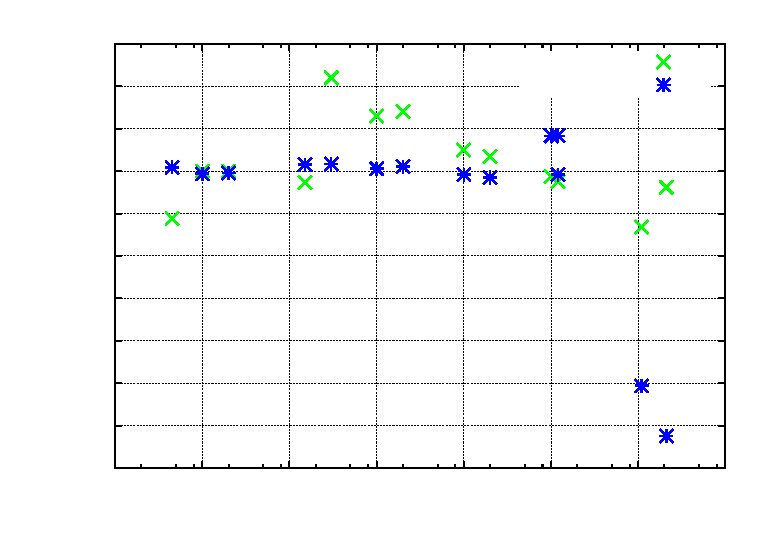
\includegraphics{../GNU/induct328p}}%
    \gplfronttext
  \end{picture}%
\endgroup

\caption{Induktivit\"ats-Messfehler von 15 verschiedenen ATmega}
\label{fig:Induct328p}
\end{figure}
